\documentclass[fleqn]{article}

\usepackage{haldefs}
\usepackage{notes}
\usepackage{graphicx}
\usepackage{rotating}
\usepackage{caption}
\usepackage{url}

\begin{document}
\lecture{01/12/12}{ProseVis User and Developer Specifications}{Megan Monroe, Ankita Garg}

\section{Overview}

The ProseVis visualization tool provides analysts with the ability to explore and understand the phonetic elements of a given text.  While certain features allow for analysis at the text level, the focus of the tool is on the way that the text sounds when it is spoken aloud.  Features for this phonetic analysis are computed by the Open Mary text-to-speech system.  

\section{User Specs}
This section details the features of ProseVis, as seen by the user.  It describes the various manipulations that can be performed on the text.  A graphic, illustrating the elements of the interface, can be found at the end of the document.

\subsection{File Management}
ProseVis supports the analysis of at most two concurrent files.  Files can be opened and closed using the top file menu, and can be tiled either horizontally or vertically in the visualization panel according to the user's preference.  Compatible files must conform to the output of the Open Mary text-to-speech system which, most generally, are tab delimited text files.  For a more detailed description of the input files and their generation, please see the file management section in the Developer Specs.

\subsection{Navigation Panel}
The navigation panel provides a persistent, zoomed out view of the visualization.  In a typical setting, the user will be zoomed into a specific section of a given document.  The navigation panel allows the user to maintain the context of where they are in the entire document.

\subsection{Render Options}
The rendering options on the data panel provide the primary means of manipulating the visualization.  These options include:

\subsubsection*{Zoom}
The initial visualization is presented at 25\% of it's normal size, to present a fish-eyes view of the file, with a minimum font size of 2. This ensures that large files can be displayed properly. The user then has the option of increasing the visualization to up to 800\% of it's normal size.

\subsubsection*{Line By}
The visualization renders a given document as a series of lines (rows).  The breakpoints of these lines can be determined by any level in the document hierarchy.  At the highest level, the entire document can be rendered as a single line.  At the lowest level, each phrase in the document is rendered as its own line.

\subsubsection*{Color By}
For every attribute of the document (word, sound, accent, etc.) ProseVis maintains a list of unique occurrences.  For example, a list of every unique word in a given document is maintained internally.  The user can choose to color the visualization by any of these attributes.  

If the user chooses to color the visualization by the sound, they have the additional option of coloring by the full sound, or by a component of the sound.  Sounds are presented in the input files as a space delimited series of consonant and vowel components.  The components of the sound that can be targeted for color include the leading consonant, the vowel, and the ending consonant.  The user should also keep in mind that some sounds lack one or more of these components, and the absence of any such component will be assigned a color as well.  An example sound breakdown follows:
\\
\begin{table}[h]
\centering
\begin{tabular}{| r | c || c | c | c | }
\hline
Word & Sound & Lead Consonant & Vowel Sound & End Consonant\\
\hline
Strike & s tr I ke & s & I & ke \\
\hline
\end{tabular}
\caption*{Sound Breakdown}
\end{table}

The possible vowel and consonant components can be found at: \\
http://mary.opendfki.de/wiki/USEnglishSAMPA\\
\\
However, over the course of testing ProseVis, we uncovered two additional vowel components, {\bf @U} and {\bf EI}, which are now included in the implementation.  It is also worth pointing out that nearly every sound contains a vowel component.  Across the three files that we analyzed during testing, we only found four words that contained a sound that did not include a vowel component.  The words were:\\

Struggle, Skeene, Stay, Stayed\\
\\
In all four of these words (which accounted for 67 instances across all three files), the leading `S' was separated into it's own sound.

\subsubsection*{Render}
The user has the option to render many different types of text in the visualization. The text rendered can either be the actual words in the document, the sounds that comprise each word, or the part-of-speech of each word.  If the user chooses not to render any of this text, the visualization will render the document as a sequence of equally sized blocks, where each block corresponds to a single sound.  These blocks will be grouped and outlined by word.

\subsubsection*{Accent}
Accent is rendered graphically according the pronunciation of each word.  In can be rendered in any of the above coloring or text render schemes.

\subsubsection*{Line Numbers}
The user has the option to view the line numbers or paragraph numbers, etc (depending on the selection of 'Line By') in the visualization of the text. The 'View' menubar option can be used to enable or disable line number rendering.

\subsection{Search}
The search panel allows for text-based search by either word, part-of-speech, sound, or soundex representation.  A sound-based search can be further specified by any of the sound components that were discussed previously.  The search begins at the beginning of the text and continues within the body for every click of the 'Search' button. It wraps around to the beginning once the entire file has been searched once. The line containing the search term is displayed as the very first line of the visualization. The terms are not highlighted in yellow to prevent it from overriding the 'Color By' selection.

\section{Developer Specs}
The section describes the basic architecture of the ProseVis tool from a developer's standpoint, as well as the implementation details for select features.

\subsection{File Creation}
Files are created in a two steps: processing an xml file into the Seasr database, and exporting the resulting table as a tab delimited text file.  An xml file, representing a single written work, can be processed into the Seasr database using the Meadre Workbench at:\\
\\
Site: http://demo.seasr.org:1712\\
user = admin\\
pwd = admin\
server = leovip021.ncsa.uiuc.edu\\
port = 1714 (the default)\\
\\
When the Workbench opens, the leftmost panel should display a list of flows.  Double click the flow entitled ``Process XML to OpenMary to DB", which should open this flow in the main, central panel of the workbench. If you are not able to find this flow, please contact Tanya or Loretta to get the particular flow reloaded into the workbench. Then click the button entitled ``Run Flow" in the top right corner of the main panel. The flow requires the input file. Either a pop-up window, prompting you to select a file to process will open up, or you might need to go to http://leovip021.ncsa.uiuc.edu:1715/ from your browser and specify the file you want to process. Click on submit.

The Workbench will then begin processing the file, which can take anywhere from a couple minutes to a few hours, depending on the file size.  When the run is complete, the console panel of the Workbench (typically located under the main panel) will print statistics about the run.  If the run fails, the console will display a message telling you why.  The most typical reason for a failure is that the dtd file specified in the xml cannot be found.  This can be corrected by either removing that line from the xml file, or specifying the dtd file with an absolute url.

Once the flow run is complete, the Seasr database is updated with a new table, named after the xml file name.  This table must be exported to a tab delimited text file, which can then be loaded into ProseVis.  For Mac users, the table can be easily exported using the Sequel Pro software.  This software can be installed on your computer and used to open a connection to the Seasr database using the following criteria:\\
\\
user: sound\\
pwd:  bananas\\
hostname: leovip021.ncsa.uiuc.edu\\
database: Tanya\\
\\
Once this connection is established, Sequel Pro will display a list of all the tables in the ``Tanya" database.  Right-click on the one that corresponds to the original xml file name, and click ``Export".  A window will pop up with the export options.  Change the separator option from `,' (which will produce a comma delimited text file) to `\textbackslash t' to produce a tab delimited text file.  Click ``Export" and save the file on your local system.  This file can now be opened using ProseVis.

To export the table on a Linux machine, you can use mysql to connect to the remote database server, as shown below:

\begin{verbatim}
Connect to db using mysql to confirm if the particular table has been created:
#mysql --host=leovip021.ncsa.uiuc.edu --user=sound --password=bananas Tanya
mysql> show tables \g
..
Execute the below command on your machine to export the table:
#mysql -h leovip021.ncsa.uiuc.edu -u sound -p Tanya -e "SELECT * FROM [table name]" > [output name].tsv
\end{verbatim}

Please confirm the username and password with Tanya or Loretta before using them.

\subsection{Data Structure}
Each document is processed into a tree structure comprised of nodes of the superclass, ProseNode.  A node of the tree contains links to both it's children, and it's next sibling.  The ProseNode superclass is divided into two subclasses: HierNodes and WordNodes.  The HierNodes comprise the internal structure of the tree, and contain virtually no additional information apart from structure.  HierNodes with leaf children are flagged to distinguish them from HierNodes with HierNode children.

WordNodes are used as the leaves of the tree, and contain all the pertinent information for a given word.  Though not explicitly part of the tree structure, each WordNode contains a list of Syllables, each of which contains the Syllable-specific attributes such as sound and stress.  The syllables are entirely encompassed by the word, and are not sibling-linked like the HierNodes and WordNodes.  

\subsection{Tree Iterator}
The iterator is a helper class that allows the visualization class to quickly access pertinent information.  The iterator works according to the following process:

\begin{enumerate}
\item The iterator is initialized with a parent node (HierNode) to traverse.
\item The rightmost {\bf leaf} of the designated parent node is flagged as the stopping point.
\item The iterator's Next method returns sequential WordNodes, beginning with the parent node's leftmost leaf.
\item The iterator returns null when the stopping point is reached.
\item The stopping point flag is removed from the the appropriate WordNode.
\end{enumerate}

\subsection{Input Files}
Each opened document is parsed into the InputFile class.  This class is the internal representation of the document, and maintains the list of unique occurrences for each attribute, as well as a list of the leftmost nodes at each level of the tree.  When more than one file is opened, the attribute lists from the first file are incorporated into the second file so as to maintain consistent indices for each occurrence across all attributes.  

\subsection{Visualization}
The visualization is drawn in two steps.  The first step, prepVis, is performed by the single VizController class that handles the overall layout computations, determining the placement, size, and font size for each document.  Once these parameters are determined, each individual Visualization class renders it own panel.

\begin{sidewaysfigure}[p]
  \begin{center}  
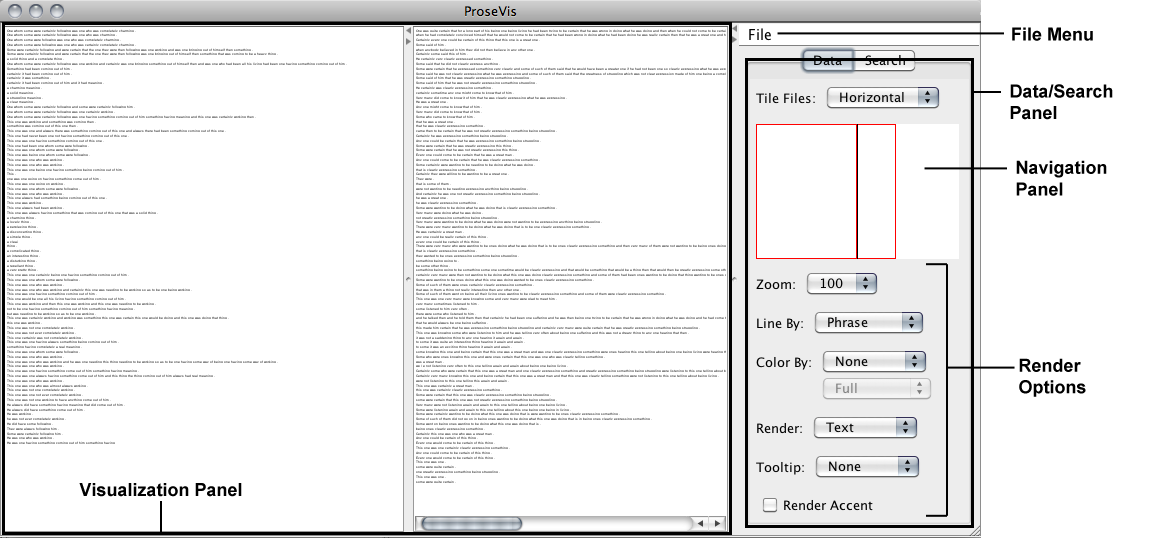
\includegraphics[scale=.5] {ProseVisImg.png}
\end{center}
\caption{The ProseVis User Interface }
 \end{sidewaysfigure}

\section{Java Heap Size}
ProseVis requires a much larger heap size for manipulating large files. It has been observed that a typical heap size of 1.5-2GB is needed to handle files of sizes greater than 250-300MB. One can increase the default heap size by running the jar from the commandline and specifying the '-Xmx' parameter to the java command. To allow automating this for MAC, use the Java Bundler application on MAC to package the jar file and edit the Info.plist file to change the default JAVA heap size.

\section{Predictive Modeling}
A group of texts have been compared against each other to compute the probablity of every phoneme in a given text file occuring in the other files in the group. At present, ProseVis aids in the comparison of 9 text files that have been pre-defined. The input text files have probability data for every syllable in the file for every other file. At the time of opening a file, all the probability values are read in. The different file names are displayed in the 'Comparison' tab. For the files that have been selected in this tab, every phoneme is colored with a shade of the color corresponding to the file that has the most occurence of that phoneme. The intensity of the shade determines the extent to which there is a resemblence or confusion in prediction of likelyhood. For example, if a file A is compared against B and C, and if C has the highest occurrence of a particular phoneme, but if it is not been selected for comparison, the phoneme is colored with the color of file B with a slightly lighter shade.

The DavidData class models the probability of every phoneme and computes the relative and maximum probability values, which are used for the computation of the intensity of the color used for display. Also, a list of files being compared against is maintained to determine the relative probabilities.

\end{document}